\documentclass[11pt,a4paper]{article}
\usepackage[margin=2.4cm]{geometry}
\usepackage[T1]{fontenc}
\usepackage{lmodern}
\usepackage{amsmath,amssymb}
\usepackage{booktabs}
\usepackage{graphicx}
\usepackage{siunitx}
\usepackage{microtype}
\usepackage{xcolor}
\usepackage{pgfplots}
\pgfplotsset{compat=1.18}
\usepackage[hidelinks]{hyperref}
\sisetup{group-separator={,},group-minimum-digits=4}
\newcommand{\cfg}[1]{\texttt{#1}}
\setlength{\parskip}{0.3em}
\setlength{\emergencystretch}{2em}
\definecolor{s1}{HTML}{2a78d6}
\definecolor{s2}{HTML}{eb6834}
\definecolor{s3}{HTML}{1baf7a}
\definecolor{inkmuted}{HTML}{6b6a64}

\begin{document}

\begin{center}
  {\LARGE Sonar debris detector: one evaluation protocol,\\[0.2em]
  and MCNN under the same conditions}\\[0.6em]
  {\large Project report, \texttt{sonar\_edge}, second round}\\[0.3em]
  11 November 2026
\end{center}
\vspace{0.5em}

\section*{Scope}

This report answers the points raised on the deployment report
(\texttt{report/deployment.pdf}). Each point and where it is treated:

\begin{enumerate}
  \item The 5-fold figure (52.6 mAP) and the Raspberry Pi figure (63.8 mAP)
        were not comparable. All five fold models of both configurations,
        three seeds each, have now been run on the Pi, so every accuracy
        figure below is a pooled 5-fold result
        (Section~\ref{sec:protocol}).
  \item MCNN should be compared with the detector under the same test
        conditions, for accuracy and for speed. MCNN was retrained on the same
        scene folds, the detector was scored on MCNN's task, and both were
        timed on the Pi in the same inference framework
        (Sections~\ref{sec:mcnn} and~\ref{sec:speed}).
  \item Thermal tests: a short note on whether they are needed
        (Section~\ref{sec:thermal}).
  \item A Raspberry Pi~5 comparison, to show the hardware dependence
        (Section~\ref{sec:pi5}).
  \item External validation on similar data: what public data exist and
        what each would allow (Section~\ref{sec:external}).
  \item Whether the test results can be raised (Section~\ref{sec:improve}),
        and the framing as a lightweight detector
        (Section~\ref{sec:framing}).
\end{enumerate}

One figure of the deployment report is corrected here: the per-frame cost
of MCNN (Section~\ref{sec:speed}).

\tableofcontents

% ---------------------------------------------------------------------------
\section{One accuracy protocol, measured on the device}
\label{sec:protocol}

\subsection{Why 52.6 and 63.8 differed}

The frames of the dataset are grouped into \emph{scenes}: runs of frames
with the same objects in the same places. The scenes are distributed over
five folds. In 5-fold cross-validation, five models are trained; model $k$
is tested on fold $k$, validated (for choosing the training epoch) on fold
$(k+1) \bmod 5$, and trained on the other three. Every frame is thus tested
exactly once, by a model that has never seen its scene.

The 52.6 is the \emph{pooled} result: the test detections of all five models
are put together and scored as one detection problem over all \num{1868}
frames, and the figure is the mean of three training seeds. The 63.8 was a
single model (seed~0, fold~0) on its own test fold of 439 frames. Folds
differ a great deal in difficulty, because each holds different scenes and
some classes sit almost entirely in one fold (61 of the 65
\emph{standing-bottle} boxes are in fold~3, 158 of the 240 \emph{valve}
boxes in fold~2). Fold~0 is one of the easy folds: the same model scores
63.8, 65.4, 51.5, 44.7 and 66.2 on folds 0 to 4. The two numbers therefore
measured different things, and only the pooled one describes the method.

\subsection{Method}

For both configurations at $360 \times 240$ input (\cfg{small}, the
deployed one, and \cfg{small\_wide}, the more accurate one), all
$2 \times 3 \times 5 = 30$ fold models were exported to C, built natively
on the Pi with the NEON kernel, checked with the golden test (all 30
passed), and run over their own test folds. The detections were copied to
the laptop and scored with the same code as the Python models
(\texttt{c\_eval --pred}), then pooled over folds (\texttt{sonar-edge cv},
new variant \texttt{pi4}).

\subsection{Results}

\begin{table}[h]
\centering
\caption{Detection mAP@0.5 under 5-fold scene cross-validation, mean of
three seeds. ``Pooled'' scores all \num{1868} test frames together; the
fold columns are each fold's own mAP (mean of seeds). Float: PyTorch model;
int8: Python integer reference; Pi~4: C runtime on the device.}
\label{tab:cv}
\resizebox{\textwidth}{!}{\begin{tabular}{llcccccc}
\toprule
Model & Run on & Pooled & Fold 0 & Fold 1 & Fold 2 & Fold 3 & Fold 4 \\
\midrule
\cfg{small} @360  & float (GPU)    & $52.6 \pm 1.9$ & 61.0 & 65.1 & 52.2 & 48.2 & 67.5 \\
                  & int8 (Python)  & $52.3 \pm 1.7$ & 59.5 & 64.5 & 52.0 & 47.4 & 66.0 \\
                  & int8 (Pi~4)    & $\mathbf{52.3 \pm 1.7}$ & 59.5 & 64.5 & 52.0 & 47.5 & 66.0 \\
\midrule
\cfg{small\_wide} @360 & float (GPU)   & $56.9 \pm 2.7$ & 67.7 & 68.0 & 58.1 & 52.0 & 70.9 \\
                  & int8 (Python)  & $56.7 \pm 2.6$ & 66.5 & 66.6 & 58.1 & 52.6 & 69.9 \\
                  & int8 (Pi~4)    & $\mathbf{56.7 \pm 2.7}$ & 66.5 & 66.6 & 58.1 & 52.6 & 69.9 \\
\bottomrule
\end{tabular}}
\end{table}

The device reproduces the integer reference to the first decimal on every
fold and in the pooled figure; the per-seed pooled values on the Pi are
53.7, 52.8, 50.4 (\cfg{small}) and 58.8, 53.7, 57.7 (\cfg{small\_wide}).
Differences of a few hundredths of a point between the two int8 rows come
from the C program's lower score threshold for emitting a detection, not
from the network, whose outputs are bit-identical (golden test). The
accuracy to quote for the deployed system is therefore
\textbf{52.3~mAP} (\cfg{small}) or \textbf{56.7~mAP} (\cfg{small\_wide}),
measured on the Pi. The 63.8 should not be used except as ``fold~0''.

% ---------------------------------------------------------------------------
\section{MCNN under the same conditions: accuracy}
\label{sec:mcnn}

\subsection{The two tasks}

MCNN and the detector do not solve the same problem. MCNN is a
\emph{classifier}: it receives one object, already cut out of the sonar
frame along its annotated bounding box and zero-padded to $305 \times 305$
pixels, and outputs one of ten classes. Someone must have found the object
and drawn the box before MCNN runs. The detector receives the whole frame
and must both find the objects and name them.

A direct comparison therefore needs a common task. The only task both can
perform is MCNN's: \emph{given the annotated objects, name them}. MCNN is
handed the boxes; the detector is not, and is scored on whether it finds
each annotated object and names it correctly. This favours MCNN, and the
comparison should be read with that in mind.

\subsection{MCNN trained on the scene folds}

The published MCNN accuracy (and the 99.8\,\% of our reimplementation in
\texttt{sonar\_cnn}) comes from a random 80/20 split of the
\texttt{watertank-cropped} set. That split places near-identical frames of
the same scene on both sides, and in the reimplementation report a
nearest-neighbour lookup on $32 \times 32$ thumbnails alone reached 100\,\%
on it. To put MCNN under the detector's conditions:

\begin{itemize}
  \item \textbf{Data.} Every annotated box of the ten object classes
        (\emph{Wall} excluded, as in the cropped set used by the paper) was
        cut from the full $320 \times 480$ frames at native resolution: \num{2826}
        crops, the largest $299 \times 253$, so the paper's zero-padding to
        $305 \times 305$ applies without resizing. These are not the same
        images as \texttt{watertank-cropped} (\num{2364} crops, cut by the
        dataset authors), but the same objects in the same recordings.
  \item \textbf{Split.} Each crop inherits the fold of its frame. Fold $k$
        test, fold $(k+1) \bmod 5$ validation, the other three training,
        as for the detector.
  \item \textbf{Training.} As in the reimplementation: AdamW, learning rate
        $10^{-3}$, weight decay $10^{-4}$, cosine schedule, 30 epochs,
        batch 32. The epoch with the best validation accuracy is kept, as for
        the detector. Three seeds.
  \item \textbf{Metric.} Accuracy over the pooled test predictions of all
        five folds (each crop tested once), and macro-F1, the mean over the
        ten classes of the F1 score, which weighs rare classes equally.
\end{itemize}

Code: \texttt{src/sonar\_edge/mcnn\_cv.py} (the network is a copy of the
\texttt{sonar\_cnn} implementation). Training takes about 15~s per fold on
the GPU.

\subsection{The detector on MCNN's task}

For each annotated object, the detector's answer is the class of its
highest-scoring detection that overlaps the object's box with an
intersection-over-union of at least 0.5. An object with no such detection
counts as an error (``missed''); a detection labelled \emph{Wall} counts as
an error. The detections are the on-device ones of
Section~\ref{sec:protocol}. Code: \texttt{src/sonar\_edge/gt\_cls.py}.

\subsection{Results}

\begin{table}[h]
\centering
\caption{Naming the \num{2826} annotated objects, 5-fold scene CV, mean $\pm$
standard deviation over three seeds. MCNN is given each object's box; the
detectors must find it (``missed'': no detection overlaps the box).}
\label{tab:cls}
\resizebox{\textwidth}{!}{\begin{tabular}{lccccccccc}
\toprule
Model & Boxes given & Accuracy & Macro-F1 & Missed & \multicolumn{5}{c}{Accuracy per fold} \\
\cmidrule(lr){6-10}
 & & (\%) & (\%) & (\%) & 0 & 1 & 2 & 3 & 4 \\
\midrule
MCNN                    & yes & $77.7 \pm 0.5$ & $71.4 \pm 1.7$ & --  & 84.5 & 89.6 & 47.0 & 83.6 & 78.5 \\
\cfg{small} @360        & no  & $74.2 \pm 1.3$ & $70.4 \pm 3.0$ & 7.4 & 83.8 & 85.1 & 55.4 & 62.1 & 70.8 \\
\cfg{small\_wide} @360  & no  & $77.6 \pm 2.4$ & $74.4 \pm 2.7$ & 6.3 & 85.7 & 88.8 & 63.0 & 68.7 & 70.3 \\
\bottomrule
\end{tabular}}
\end{table}

\paragraph{MCNN without leakage.} Under scene folds MCNN reaches 77.7\,\%,
not 99.8\,\%. The 22-point gap is the effect of the split: on a random
split the test frames are near-copies of training frames, so the score
measures recall of seen scenes rather than recognition of objects in new
ones. This is the main methodological finding for the paper.

\paragraph{Detector against MCNN.} Although it is not told where the objects
are, \cfg{small\_wide} matches MCNN in accuracy (77.6 against 77.7) and
exceeds it in macro-F1 (74.4 against 71.4); \cfg{small}, with 66 times fewer
parameters than MCNN, is 3.5 points lower in accuracy and 1 point lower in
macro-F1. Between 6 and 8\,\% of objects are not found at all, so among the
objects the detectors do find, their naming is more accurate than MCNN's.
The seed-to-seed spread of the detectors (1.3 to 3.0 points) is as large as
most of these differences; the only firm statements are that the detectors
are on a par with MCNN on its own task and that \cfg{small\_wide} is not
worse in any aggregate.

\paragraph{Where they differ.} Figure~\ref{fig:recall} shows the share of
each class named correctly. MCNN is better on \emph{can}, \emph{chain} and
\emph{standing-bottle}; the detectors are better on \emph{shampoo-bottle}
and \emph{valve}. Two observations explain most of this:

\begin{itemize}
  \item MCNN sees the box outline, and with it the object's size and aspect
        ratio. In the reimplementation report a random forest on crop
        height and width alone reached 98\,\% on the random split. A
        standing bottle has a distinctive tall, narrow box, and nearly all
        of them are in fold~3; this is where MCNN gains most (fold~3: 83.6
        against 62--69). With the box given, part of the classification is
        done by the annotator.
  \item Fold~2 holds two thirds of all valves, so the models tested on it
        are trained on only 69 valves. MCNN names 17\,\% of the fold-2
        valves correctly and drops to 47\,\% on that fold; the detectors,
        which see the valves' surroundings, drop less (55--63\,\%).
\end{itemize}

\begin{figure}[h]
\centering
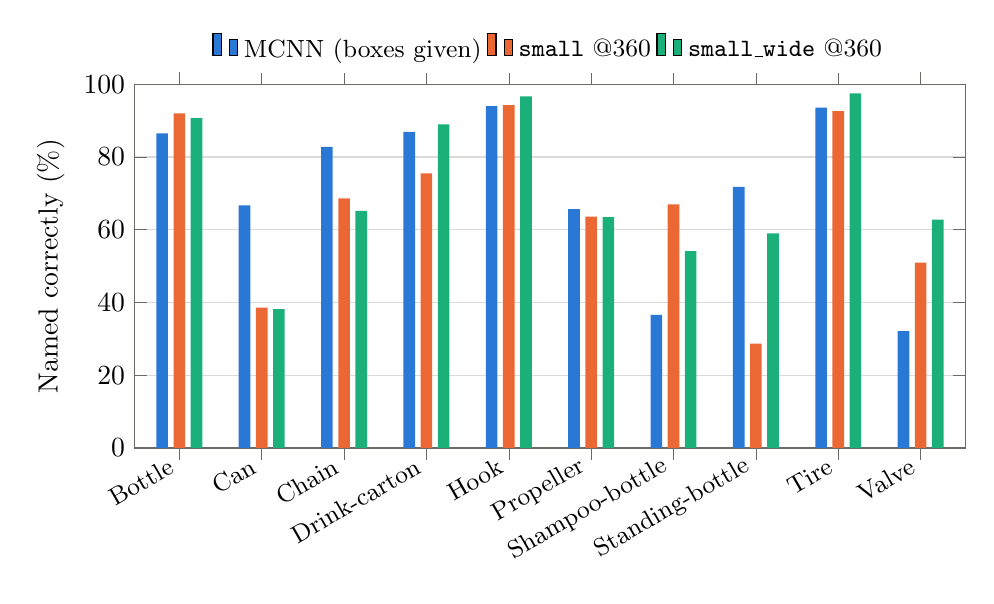
\begin{tikzpicture}
\begin{axis}[
  ybar, bar width=4.2pt, width=\textwidth, height=6.2cm,
  ymin=0, ymax=100, ylabel={Named correctly (\%)},
  symbolic x coords={Bottle,Can,Chain,Drink-carton,Hook,Propeller,Shampoo-bottle,Standing-bottle,Tire,Valve},
  xtick=data, x tick label style={rotate=30, anchor=east, font=\small},
  ymajorgrids, grid style={inkmuted!25}, axis line style={inkmuted}, tick style={inkmuted},
  legend style={at={(0.5,1.03)}, anchor=south, legend columns=3, draw=none, font=\small},
  enlarge x limits=0.06,
]
\addplot[fill=s1, draw=none] coordinates {(Bottle,86.5) (Can,66.7) (Chain,82.8) (Drink-carton,86.9) (Hook,94.0) (Propeller,65.7) (Shampoo-bottle,36.6) (Standing-bottle,71.8) (Tire,93.6) (Valve,32.1)};
\addplot[fill=s2, draw=none] coordinates {(Bottle,92.0) (Can,38.6) (Chain,68.6) (Drink-carton,75.5) (Hook,94.3) (Propeller,63.6) (Shampoo-bottle,67.0) (Standing-bottle,28.7) (Tire,92.6) (Valve,51.0)};
\addplot[fill=s3, draw=none] coordinates {(Bottle,90.7) (Can,38.2) (Chain,65.2) (Drink-carton,89.0) (Hook,96.7) (Propeller,63.5) (Shampoo-bottle,54.1) (Standing-bottle,59.0) (Tire,97.5) (Valve,62.8)};
\legend{MCNN (boxes given), \cfg{small} @360, \cfg{small\_wide} @360}
\end{axis}
\end{tikzpicture}
\caption{Per-class recall on the naming task (Table~\ref{tab:cls}), mean of
three seeds, pooled over the five folds. Class sizes: 468, 292, 320, 347,
171, 197, 111, 65, 615 and 240 objects.}
\label{fig:recall}
\end{figure}

% ---------------------------------------------------------------------------
\section{MCNN under the same conditions: speed and memory}
\label{sec:speed}

\subsection{Method}

The detector runs on the Pi in our integer C runtime; MCNN has no such
implementation. Timing the two in different software would compare the
software as much as the networks. Both were therefore exported to ONNX and
run in the same general-purpose engine, ONNX Runtime~1.31.1 (32-bit floating
point, CPU), on the same Pi~4, with one thread and with four. Each
measurement is 10 warm-up runs and then 3 repeats of 50 runs; the three
repeats agree within 1.5\,\%, and the mean is reported. The network
computation does not depend on the image content, so random inputs of the
right size were used. Memory is the process's peak resident size
(\texttt{VmHWM}); an interpreter with ONNX Runtime loaded and no model uses
45.5~MB, which is included in every ONNX figure.

MCNN's cost per frame depends on how many objects the frame holds. The
dataset has \num{2826} non-\emph{Wall} objects in \num{1868} frames,
1.51 per frame on average (at most 4; 68 frames have none). Two crops in one
batch take exactly twice as long as one (130.7 against 66.5~ms), so the
per-frame time is 1.51 times the per-crop time.

\subsection{Results}

\begin{table}[h]
\centering
\caption{Cost on the Raspberry Pi~4. ONNX Runtime columns: float32, same
engine for all models. C runtime: our int8 runtime with the NEON kernel,
one thread (deployment report). MCNN per frame = 1.51 crops.}
\label{tab:speed}
\resizebox{\textwidth}{!}{\begin{tabular}{lrrrrrrr}
\toprule
 & & & \multicolumn{3}{c}{ONNX Runtime, ms} & C int8 & Peak memory \\
\cmidrule(lr){4-6}
Model & Params & MMAC/frame & & 1 thread & 4 threads & ms & ONNX / C (MB) \\
\midrule
MCNN       & \num{2797706} & 355 & per crop  & 66.5  & 24.7 & --   & 75.5 / -- \\
           &               &     & per frame & 100.6 & 37.4 & --   &  \\
\cfg{small} @360       & \num{42463}  & 78  & per frame & 22.4 & 8.8  & 20.3 & 58.1 / 2.3 \\
\cfg{small\_wide} @360 & \num{135359} & 204 & per frame & 48.7 & 17.2 & 46.5 & 58.7 / 2.6 \\
\bottomrule
\end{tabular}}
\end{table}

\paragraph{Same engine.} In the same software, the deployed detector
processes a whole frame 4.5 times faster than MCNN classifies the objects
in it (22.4 against 100.6~ms, one thread), and 3.0 times faster than MCNN
classifies a single crop. \cfg{small\_wide}, whose naming accuracy equals
MCNN's, is 2.1 times faster per frame. These figures still leave out the
step that MCNN needs and the detector does not: finding the objects. Any
proposal stage added in front of MCNN adds its own time.

\paragraph{Correction.} The deployment report gave MCNN's per-frame cost as
490~M multiply-accumulates, using 2.08 objects per frame. That count
included the \emph{Wall} boxes, which MCNN does not classify. The correct
figure is $234.7 \times 1.51 = 355$~M, 4.5 times the detector's 78.4~M,
which agrees with the measured time ratio.

\paragraph{What the C runtime adds.} The ONNX Runtime timings show that the
speed of the deployed detector does not come mainly from our runtime: on
one core, ONNX Runtime in floating point runs it in 22.4~ms, our int8 NEON
runtime in 20.3~ms. The speed comes from the network's size. The C runtime
contributes elsewhere: the whole program needs 2.3~MB of memory instead of
58~MB, has no dependency beyond the C standard library (no Python, no
inference engine), stores its weights in 42~KB, and produces output that is
bit-identical on every platform, so the cross-validated accuracy holds on
the device by construction. ONNX Runtime with four threads uses all cores for
one frame (8.8~ms); our runtime is single-threaded and uses the four cores
by running four copies (187 frames/s in total, 21~ms each). An int8 ONNX
model was not tried.

% ---------------------------------------------------------------------------
\section{Thermal tests}
\label{sec:thermal}

They can be dropped as a separate topic. At the deployed operating point
(one core, 20~ms per frame) the board stays near 60\,$^\circ$C without a
fan. Only four cores fully loaded with the largest model
($480 \times 320$, 450~M MACs) reached the 80\,$^\circ$C soft limit. One
sentence in a paper suffices: sustained four-core operation needs a heat
sink.

% ---------------------------------------------------------------------------
\section{Raspberry Pi 5}
\label{sec:pi5}

The Pi~5 has Cortex-A76 cores at 2.4~GHz, which implement ARMv8.2 including
the \texttt{sdot}/\texttt{udot} instructions: each multiplies four pairs of
8-bit values and adds them in one step, four times the work per instruction
of the 16-bit multiply-add the Pi~4 kernel uses. The current program runs
on the Pi~5 unchanged (it would use the Pi~4 NEON kernel), and a second
kernel using the dot-product instructions can be added behind a compile-time
check. A Pi~5 would give three data points (laptop x86, Pi~4, Pi~5) for the
same bit-identical program: the same accuracy and three latencies, which
shows the hardware dependence directly. The measurement scripts are ready;
it takes about an hour once a board is reachable over the network.

% ---------------------------------------------------------------------------
\section{External validation}
\label{sec:external}

The dataset comes from the public \texttt{marine-debris-fls-datasets}
collection (Valdenegro-Toro et al.), which holds three further sets recorded
with the same sonar (ARIS Explorer~3000). None is a ready-made external
detection test:

\begin{itemize}
  \item \textbf{Quarry} (about \num{7200} full-size frames, flooded quarry, real
        water): the closest to field use, but released without bounding boxes
        (it is intended for unsupervised learning). Usable for a qualitative
        test (detections drawn on frames), or quantitatively after labelling
        a subset by hand.
  \item \textbf{Turntable} (crops, 12 object classes): objects on a rotating
        platform, viewed from all angles. Several classes overlap with ours
        (can, drink carton, bottles, tyres, propeller, valve). It contains
        crops, not frames, so it suits an external test of the classifier
        (MCNN) rather than the detector.
  \item \textbf{UATD} (Xie et al., \emph{Scientific Data} 2022): a different
        sonar (Tritech Gemini 1200ik), lake and shallow sea, over \num{9000}
        frames with boxes, 10 classes of which only the tyre overlaps with
        ours. Usable for class-agnostic detection or for a fine-tuning
        experiment, which tests the method on a new sensor rather than the
        trained model.
\end{itemize}

A reasonable order: a qualitative run on the quarry frames first (no labels
needed, and it shows how a tank-trained model behaves in real water), then
a decision on labelling a quarry subset.

% ---------------------------------------------------------------------------
\section{Can the test results be raised?}
\label{sec:improve}

Ranked by expected effect per effort:

\begin{enumerate}
  \item \textbf{Deploy \cfg{small\_wide}.} +4.4 pooled mAP (56.7 against
        52.3 on the device), equal to MCNN on its own task, 46.5~ms per frame
        (21.5 frames/s). Already measured; it needs only a change of the
        shipped weights.
  \item \textbf{Knowledge distillation.} Train the small network to imitate
        the larger $480 \times 320$ model's output maps in addition to the
        labels. This often recovers part of the gap between a large and a
        small network without changing the deployed cost.
  \item \textbf{The weak classes.} \emph{Can} (38\,\% named correctly by the
        detectors, 67\,\% by MCNN), \emph{standing-bottle} and \emph{valve}
        are limited by the data: the latter two sit almost entirely in one
        fold, so the model tested on that fold has seen few examples.
        Class-balanced sampling or copy-paste augmentation of rare objects
        into other scenes addresses this directly.
\end{enumerate}

Wider networks beyond \cfg{small\_wide} were not better: a 48-channel
variant scored 50.9 pooled mAP (one seed).

% ---------------------------------------------------------------------------
\section{Framing}
\label{sec:framing}

The results support presenting the work as a lightweight object detector
for forward-looking sonar, along the lines of the proposed title
\emph{Efficient Marine Debris Detection in Forward-Looking Sonar Images
Using a Lightweight Neural Network}. The advantages, with the figures that
back them:

\begin{itemize}
  \item \textbf{Raw frames in.} A remotely operated or autonomous vehicle
        receives whole sonar frames, not cropped objects. The detector
        takes the frame as it comes ($360 \times 240$ after
        resizing) and needs no separate stage to find and crop objects.
        A crop classifier such as MCNN is only half of a system.
  \item \textbf{One pass.} One forward pass finds and names every object:
        78~M MACs, against 355~M for MCNN to name the objects of an average
        frame once they have been found.
  \item \textbf{Embedded.} 20.3~ms per frame on one Pi~4 core (49 frames/s;
        187 frames/s on four), 2.3~MB of memory, \num{42463} parameters
        (66 times fewer than MCNN), no dependencies, and accuracy on the
        device identical to the cross-validated accuracy.
  \item \textbf{Honest evaluation.} Scene-level 5-fold cross-validation.
        Under it MCNN drops from 99.8\,\% to 77.7\,\%, which shows how much
        the published figure owes to the split.
\end{itemize}

% ---------------------------------------------------------------------------
\section{Limitations}

\begin{itemize}
  \item The naming comparison is between a classifier given the true boxes
        and detectors that are not; it cannot be made symmetric without a
        proposal stage for MCNN, which the paper does not define.
  \item MCNN was trained with the reimplementation's recipe (30 epochs, no
        augmentation); a longer or augmented schedule might raise it. The
        detectors use their own tuned recipe.
  \item MCNN was timed in floating point in ONNX Runtime only; an int8
        version was not built, nor was an int8 ONNX detector.
  \item Three seeds per configuration; differences under about 3 points are
        within seed variation.
  \item No external data were evaluated yet (Section~\ref{sec:external}).
\end{itemize}

% ---------------------------------------------------------------------------
\section{Summary}

\begin{itemize}
  \item All accuracy figures are now pooled 5-fold results measured on the
        Pi: \textbf{52.3~mAP} for the deployed \cfg{small} and \textbf{56.7}
        for \cfg{small\_wide}, identical to the integer reference. The
        earlier 63.8 was fold~0 alone.
  \item MCNN under the same scene folds: 77.7\,\% accuracy (99.8\,\% on the
        leaky random split). On MCNN's task, with the boxes withheld, the
        detectors reach 74.2\,\% (\cfg{small}) and 77.6\,\%
        (\cfg{small\_wide}); macro-F1 70.4 and 74.4 against MCNN's 71.4.
  \item Same engine on the Pi: the deployed detector processes a frame in
        22.4~ms; MCNN needs 100.6~ms to classify the objects of an average
        frame. The int8 C runtime (20.3~ms) adds a 25-fold memory reduction,
        no dependencies, and exactness rather than speed.
  \item Next: Pi~5 (needs a board), a qualitative test on the quarry frames,
        and distillation or rare-class augmentation to raise the scores.
\end{itemize}

\end{document}
